%% content.tex
%%

%% ================================================================================================================================================================

\chapter{Abstract}

In unser heutigen hoch technologisierten Welt steigt stetig und rasant die Leistungsfähigkeit moderner Grafikhardware.
Um heutzutage Grafik auf einem modernen Computer darzustellen sind mittlerweile eine Vielzahl von Zwischenschritten nötig.
Diese Arbeit beschäftigt sich um die einzelnen Stufen dieser Kette, deren jeweilige Aufgabe, ihren Datentransfer untereinander,
ihre Reihenfolge sowie ihren Arbeitskontext. Beim Arbeitskontext werden unter anderem die unterschiedlichen Koordinatensysteme untersucht. 
Dabei soll nicht nur konkret auf die Arbeitsweise der einzelnen Stufe eingegangen werden, sondern auch im Speziellen auf die Zusammenarbeit und Kommunikation. 
Exemplarische Fragestellungen die behandelt werden sind Folgende: Können in dieser Art der Abarbeitung Flaschenhälse entstehen und 
wie werden Sie umgangen bzw. bekämpft. Welchen Einfluss hat der Programmierer auf die Pipeline bzw. welche Schritte kann er selber
implementieren und welche Schritte werden rein von der Hardware übernommen und können nicht von ihm modifiziert werden. 
Diese Arbeit macht den Aufbau einer modernen Rendering-Pipeline verständlich und vermittelt den Begriff Rasterisierung
Zusätzlich wird es bei dieser Abhandlung, dank des stetigen technologischen Fortschritts, ein Ausblick auf zukünftige Entwicklungen
und Neuerungen gegeben, die zukünftig moderne Rendering-Pipelines beherrschen wird.
%% ================================================================================================================================================================

\chapter{Einleitung}

Wollen wir mit einer Anwendung~\ref{sec:Anwendung} eine Szene von Objekten, z.B. eine Teekanne in einem Stadion, auf einem Computer darstellen, 
so liegt das Objekt zuerst in Form von vielen Eckpunkten(Dreiecken, Linien) in der Anwendung vor. Dabei befinden wir uns im "Model Space".
Wollen wir die Teekanne innerhalb unserer Welt (das Stadion) bewegen, wenden wir auf jede Koordinate des Modells(gemeint sind alle mit dem Modell
assoziierten Eckpunkte, Normalen) den "Model Transform" an und gehen somit in den "World Space". Die geschieht meist in der Anwendung bevor die Geometrie
zur Geometriestufe~\ref{sec:Geometry Stage} geschickt wird. \par
Als Anwender können wir nun zu Beginn der Geometriestufe mit einem eigenen Vertex Shader die Beleuchtungsberechnung etc. der Eckpunkte bestimmen. Dabei
helfen die von der Anwendung mitgegebenen Attribute. Auch in welchen Koordinatensystem dies geschieht bleibt dem Programmierer überlassen. In der anschließenden 
Stufe werden diese Eckpunkte zu Primitiven zusammengesetzt und können weiter unterteilt werden~\ref{subsec:Tessellation}.Die Primitive werden von dem Tessellation- 
zum Geometry Shader durchgereicht, welcher diese vervielfachen, entfernen oder beliebig verändern kann..\par
Um eine (orthographische oder auch perspektivische) Projektion vorzubereiten, wenden wir einen "View Transform" an. Damit können wir in den "View Space" gelangen
und vereinfachen die darauffolgende Projektion. Egal welche Art von Projektion wir angewendet haben, unsere Szene mit der Teekanne im Stadion liegt nun in einem 
Einheitswürfel. \par
Nun kann die Teekanne derart platziert sein, dass Teile außerhalb unseres Sichtfeldes(frustum) liegen. Aufgabe des Clipping~\ref{subsec:Clipping} ist nun
das "Frustum Culling", also das Abschneiden des nicht sichtbaren Bereichs, um weitere Berechnungen innerhalb darauffolgender Stufen zu beschleunigen.
Der Entwickler hat keinen Einfluss auf das Clipping~\ref{subsec:Clipping} (Abschneiden nicht relevanter Szenengeometrie). Ein Algorithmus der dieses Problem löst,
ist der Cohen-Sutherland-Algorithmus.\par
Nach dem Beschneiden liegen nur noch die "sichtbaren" Primitive vor und gelangen in die nächste Pipelinestufe, dem Viewport Transform~\ref{subsec:Viewport Transform}.
Die x-und y-Komponente unserer Eckpunktositionen werden auf die Bildschirmgröße skaliert und bilden die schlussendliche Position des Vertex. Dabei ist es wichtig 
anzumerken, dass wir die z-Komponente für weitere Berechnungen in der Rasterisierung~\ref{sec:Rasterisierung} speichern.\par
Nun sind wir an dem Punkt angelangt, an dem wir unsere transformierten, projizierten, sichtbaren Eckpunkte mit ihren Shadinginformationen vorliegen haben
(Außerdem auch Tiefenwert!). Ziel der Rasterisierung ist es nun jeden einzelnen Bildschirmpixel mit diesen Informationen einzufärben. Vor dem endgültigen Darstellen 
der Bildschirmpixel lassen sich auf den zuvor erzeuten Fragmenten eine Vielzahl von Operationen~\ref{sec:Per Fragment Operations} ausführen.So haben 
wir nun das finale Bild produziert.\par
Besonders interessant sind die neuen Shader für Ray Tracing. Die neuen Einheiten bilden eine Ergänzung der bisherigen Rasterisierung~\ref{sec:Real-Time Raytracing}.
%% ========================================================================================================================================================

\chapter{Moderne Rendering-Pipeline}

    \section{Anwendung}
    \label{sec:Anwendung}
    Zu rendernde Objekte werden zunächst von der Anwendung zur Grafikkarte geschickt. Dabei liegen die Daten über ein
    Objekt beispielhaft im OBJ-Dateiformat vor. Die Informationen über einen Vertex, das sind die Position,
    Normale und Texturkoordinate sind für Berechnungen der nächsten Stufe, des Vertex Shaders~\ref{subsec:Vertex Shader}, wichtig.
    Desweiteren werden Kamera- und Lichtposition in die Geometriestufe~\ref{sec:Geometry Stage} übergeben.
    In der Anwendung können Informationen über ein Objekt geupdatet werden, z.B. bei Kollisionen von Objekten bei denen sich 
    Positionen verändern. Allgemein werden hier Benutzereingaben gesammelt und verarbeitet.
    Als programmierbare Stufe dieser Pipeline kann der Anwender konkrete Verbesserungen in diese Stufe einbringen um z.B. mit einem BVH
    die Anzahl der Primitive für die Geometriestufe zu verrringern.
    
    \begin{figure}[H]
        \centering
        \begin{minipage}[t]{0.45\linewidth}
            \centering
            \includegraphics[width=.75\linewidth]{Bilder/MaterialDefs.PNG}
            \caption{Definition beispielhaftes Material}
        \end{minipage}
        \hfill
        \begin{minipage}[t]{0.45\linewidth}
            \centering
            \includegraphics[width=\linewidth]{Bilder/ObjectData.png}
            \caption{Vertex Daten im OBJ-Dateiformat}
        \end{minipage}
    \end{figure}

    \section{Geometrie Stufe}
    \label{sec:Geometry Stage}
        
        \subsection{Primitive Assembly}
        \label{subsec:Primitive Assembly}
        Aufgabe ist das Zusammensetzen der Eckpunkte, welche in einem Strom aus dem Vertex Shader kommen. Auf diesen Primitiven(\textit{Patches}, also
        Punkte, Linien, Drei- oder Vierecke) arbeiten die darauffolgenden Tessellation und Geometry Shader.
        So sind wir damit beispielsweiße in der Lage in nur einem Draw Call ein
        Objekt, mit möglicherweise leicht variierenden Attributen, mehrmals zu zeichnen(Instancing)

        \begin{figure}[H]
            \centering
            \def\svgwidth{\columnwidth}
            \import{Bilder/}{PrimitiveAssembly.pdf_tex}
            \label{PrimitiveAssembly}
            \caption{Buffer Objekte}
        \end{figure}

        \subsection{Vertex Shader}
        \label{subsec:Vertex Shader}
            \begin{figure}[H]
                \centering
                \def\svgwidth{\columnwidth}
                \import{Bilder/}{VertexShader.pdf_tex}
                \label{Vertex Shader}
                \caption{Funktionsweise Vertex Shader}
            \end{figure}
        Interessant zeigt sich, was direkt vor dem Aufruf des Vertex Shaders passiert: input/primitive assembling. Der Shader behandelt/verändert oder ignoriert als freiprogrammierbare Stufe 
        der Geometry Stage nur die ankommenden Vertices einzeln mit ihren Attributen (jedoch keine Erzeugung oder Löschung!!) mit Hilfe von Daten (Lichtposition, 
        Transformationsmatrix). Dabei kann kein Eckpunkt auf die Informationen eines Anderen zugreifen. Da erlaubt auch die massive parallele Ausführung auf vielen Punkten
        gleichzeitig. Mit einem Eckpunkt kommt seine Normale, Position, Farbe, möglicherweise Texturkoordinate. Ein minimalistischer Vertex Shader gibt seine Position aus.
        Dabei wechseln wir vom Modelkoordinaten zu homogenen Clipkoordinaten. Dabei kann ein Vertex Shader mehr als nur die neu berechnete Position zurückgeben. Mit krativen 
        Ansätzen lassen sich z.B. prozedurale Bewegungen nachhahmen\cite{engel2002direct3d}. Es können auch Teile der Leuchtungsberechnung ("Gouraud shading") hier angewandt werden. 
        Das Ergebnis kann zum Tessellation oder Geometry Shader geschickt werden, abgespeichert oder direkt rasterisiert werden. 
        
        
        
        \subsection{Tessellation}
        \label{subsec:Tessellation}

            \begin{figure}[H]
                \centering
                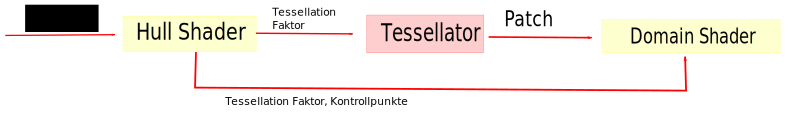
\includegraphics[width=\linewidth]{Bilder/Tessellation.pdf}
                \label{Tessellation Shader}
                \caption{Funktionsweise Tessellation Shader}
            \end{figure}

            Ist eine optionale teil-programmierbare Stufe zur Geometrieverfielfachung, d.h. eingehendes Primitiv wird weiter in viele Dreiecke unterteilt. Der \textit{Hull Shader}
            ist voll programmierbar und damit ist die Anzahl der entstehenden Dreiecke direkt beeinflussbar. Außerdem lassen sich Kontrollpunkte hinzufügen/entfernen. 
            Dabei lassen sich zwei jeweils benachbarte Patches kontrolliert unterteilen. Der \textit{Tessellator} nimmt die Patches entgegen und unterteilt Sie auf die 
            Art und Weise wie vom \textit{Hull Shader} vorgegeben. Mit dem \textit{Domain Shader} kann man jeden Vertex der vom Unterteiler kommenden Patches nachbearbeiten.
            Diese Einheit bietet den Vorteil Arbeitslast von der langsamen CPU zur schnelleren GPU zu leiten, indem man niedriger aufgelöste Meshes benutzt und diese dann 
            auf der GPU im Tessallator höher auflöst.(oder auch Meshes, welche sind schnell deformieren/bewegen). Diese Eigenschaft der Unterteilung ermöglicht auch Verfahren wie 
            Level of Detail oder Anpassungsfähigkeiten an die Leistungsfähigkeit der GPU (viele Dreiecke bei hoher Leistungskapazität).
            
        \subsection{Geometry Shader}
        \label{subsec:Geometry Shader}

            Mit dem Geometry Shader lässt sich jedes Primitiv in ein beliebiges anderes Primitiv verwandeln.

            \begin{figure}[H]
                \centering
                \def\svgwidth{\columnwidth}
                \import{Bilder/}{GeometryShader.pdf_tex}
                \label{Geometry Shader}
                \caption{Funktionsweise Geometry Shader}
            \end{figure}

            Ist wiederrum eine optionale frei-programmierbare Einheit die auf den zusammengestzten Primitiven arbeitet. Eine Vervielfachung ist theoretisch möglich,
            sollte aber als Aufgabe im Tessellation Shader erbracht werden. Vielmehr können wir diesen Shader einsetzen, um eine Geometrie gleichzeitig auf 
            mehrer rendertargets zu rendern oder wir machen transform Feedback: Buffer Objects dienen zur Speicherung von Informationen von eingehenden Primitiven.
            Diese können in weiteren Durchgängen wieder benutzt werden.
            
            \subsection{Projektionstransformation}
            \label{subsec:Projektionstransformation}    
            Die konkrete Projektion kommt erst beim Weglassen der z-Komponente. Als Vorbereitung transformieren wir unsere Eckpunkte und damit unsere Primitive in einen 
            Einheitswürfel((-1,-1,-1),(1,1,1) als Eckpunkte). Konkrete Implementierungen beziehen sich auf DirectX.
            Nehmen wir unser Sichtfeld als eine Box war, so ergibt sich eine Orthographische Transformation.
            
            \begin{center}
    
                \begin{figure}[H]
               
                    \[
                        M=
                    \left[ {\begin{array}{cccc}
                        2/(r-l) & 0       & 0       & -(r+l)/(r-l) \\
                        0       & 2/(t-b) & 0       & -(t+b)/(t-b) \\
                        0       & 0       & 1/(f-n) & -n/(f-n)     \\
                        0       & 0       & 0       & 1            \\
                    \end{array} } \right]
                    \]
                    \label{Orthographische Projektion}
                    \caption{Orthographische Projektion}
            \end{figure}
    
            Bei der orthographischen Projektion haben wir eine achsenorientierte, die Szenengeometrie umschließende Box (AABB). Aufgespannt durch Punkt
            (l,b,n) und (r,t,f).
    
            \end{center}
            
            Nehmen wir unser Sichtfeld als eine beschnittene Pyramide wahr, welche durch eine near und far plane durchzogen wird, so haben wir eine 
            perseptivische Projektion.
    
            \begin{center}
    
                \begin{figure}[H]
                    \[
                        M=
                    \left[ {\begin{array}{cccc}
                        2n/(r-l) & 0        & -(r+l)/(r-l) & 0 \\
                        0        & 2n/(t-b) & -(t+b)/(t-b) & 0 \\
                        0        & 0        & f/(f-n)      & -fn/(f-n) \\
                        0        & 0        & 1            & 0 \\
                    \end{array} } \right]
                    \]
                    \label{Perspektivische Projektion}
                    \caption{Perspektivische Projektion}
                \end{figure}
    
            \end{center}
            Near plane wird durch beide Punkte (l,b,n) und (r,t,n) aufgespannt und f ist die z-Koordinate der far plane.
            Beachte bei der perseptivischen Projektion, dass der Z-Buffer bei gößeren Distanzen ungenauer wird(kein lineares Verhalten!). So kann bei einer Szene
            mit zwei sehr nahliegenden Ebenen erst bei größerer Entfernung Z-Fighting auftreten.
         
        \subsection{Clipping}
        \label{subsec:Clipping}
        Um Objekte bzw. Objektausschnitte, welche außerhalb des Sichtfensters liegen, für die Bildsynthese zu verwerfen kommt nun das Abschneiden.
        Ein Algorithmus der dies leistet ist von Sutherland-Hodgman. Außerdem gehen wir vom Clip-Space zum Window-Space.

        \subsection{Viewport Transform}
        \label{subsec:Viewport Transform}
        
        Der auf die sichtbare Szenengeometrie reduzierte Einheitswürfel wird im diesen Schritt auf die Fenstergröße skaliert und zur Rasterisierung weitergegeben.

    \section{Rasterisierung}
    \label{sec:Rasterisierung}
    \label{sec:Fragment Shader}
            
        Zu Beginn dieser Stufe haben wir nun die Eckpunkte der bereits verarbeiteten, transformierten, projizierten Geometrie mit möglichen
        Beleuchtungsinformationen aus den vorherigen Stufen vorliegen. Zu den Window Coordinates wurde auch der Tiefenwert gespeichert. Mit der Rasterisierung
        wird nun die Farbe jedes einzelnen Pixels bestimmt. Es ist also die Aufgabe dieser Pipelinestufe herauszufinden welche Geometrie welchen Pixel zu welchen
        Anteil bedeckt und wie die Shading Informationen zur Farbgebung des Pixels beitragen.

        \begin{figure}[H]
            
\includegraphics[width=\linewidth]{Bilder/Rasterisierung.pdf}
            \label{Rasterisierung}
            \caption{Ablauf der Rasterisierung}
        \end{figure}

        Zuallererst befindet sich die Geometrie im \textit{Triangle Setup}. Unbeeinflussbar vom Programmierer werden hier Daten berechnet, welche zur Pixeleinfärbung
        benötigt werden. So werden viele zuvor per Vertex berechnete Werte interpoliert(Beleuchtung, Tiefe). Beim darauffolgenden \textit{Triangle Traversal} werden
        die wichtigen Fragmente erzeugt. Dieser Schritt bestimmt diejenigen Pixel, welche innerhalb des Dreiecks liegen und erzeugt darauf hin die Fragmente für dieses
        Dreieck anhand der zuvor berechneten/interpolierten per Dreieck Informationen. Als freiprogrammierbare Shadereinheit können im \textit{Fragment Shader}
        vom Programmierer weitere Berechnungen vorgenommen werden. Dazu zählt eine pro Pixel Beleuchtungsberechnung. Will man Texturen verwenden, so passiert das 
        nun hier.
        Das abschließende nicht komplett freiprogrammierbare, aber hoch konfigurierbare \textit{Merging} hat eine besondere Aufgabe beim Abspeichern der Farbe für
        jeden Pixel im color buffer. Zur Bestimmung der aktuellen Farbe wird nun auch das Problem der 
        Sichtbarkeit von Objekten angegangen. Zu den Z-Werten, welche wir als Tiefe beim Viewport Transform~\ref{subsec:Viewport Transform} gespeichert haben, gibt
        es hier Zugang zum Depth/Z-Buffer. Dieser Z-Buffer speichert anfangs überall den Wert inf. Beim Durchlauf der Geometrie wird nun jeweils für jeden Pixel,
        der die Geometrie bedeckt der color und depth buffer wie folgt aktualisiert: Ist der verglichene Tiefenwert des Fragmentes des Objekts kleiner als der Wert
        im Tiefenbuffer für den betroffenen Pixel, so schreibt er diesen Tiefenwert in den Z-Buffer und auch der color buffer mit der Fragmentfarbe aktualisiert.
        Anderseits passiert nichts und das nächste Primitiv wird betrachtet (Szene ohne semi-transparente Objekte!). Haben wir semitransparente Objekte, so 
        müssen wir zuerst die Szene wie beschrieben ohne diese Primitive zeichnen, alle semi-transparenten Primitive nach ihrer Tiefe ordnen und in dieser Reihenfolge 
        zu dem zuvor gerenderten Bild hinzufuegen. Damit haben wir auch unsere Projektion vollzogen, welche wir zuvor vorbereitet 
        haben~\ref{subsec:Projektionstransformation}.
        Da der buffer bereits von dem vorherigen Durchlauf Farbwerte beinhaltet ist es nun daran eine Kombination aus aktuellen Inhalt, sowie einkommende Farbe zu 
        finden, welche wiederrum im color buffer abgespeichert wird.

    \section{Per Fragment Operations}
    \label{sec:Per Fragment Operations}
        Auf den durch Rasterisierung entstandenen Fragmenten können noch einige Operationen vorgenommen werden.
        \subsection{Multisample Fragment Ops}
    
        \subsection{Stencil Test}

        Damit können wir schlussendlich entscheiden, ob ein Fragment gezeichnet werden soll oder nicht durch den Vergleich mit einem Referenzwert und 
        Stencil Buffer.(im Framebuffer).

        \subsection{Occlusion Query}
    
        \subsection{Blending}

        Wir mischen Farbwerte die bereits in den Framebuffer geschrieben wurden mit den Farbwerten, welche in den erzeugten Fragmenten vorliegen. Die Art
        in der die beiden Farben gemischt werden bestimmt eine Funktion z.B Multiplikativ, Additiv...

        \subsection{Logical Operations}

    \section{Koordinatensysteme}
    \label{sec:Koordinatensysteme}

    \section{Compute Shader}
    \label{sec:Compute Shader}

    Losgelöst von der Grafikpipeline steht der Compute Shader. Als freiprogrammierbare Einheit lässt sie sich nicht nur für graphische Berechnungen in der Pipeline, 
    sondern auch für stark parallelisierbare Probleme im Allgemeinen einsetzen. Im Folgenden wird auf die DirextX12-API~\cite[]{Direct3D12} eingegangen. 
    Der Compute Shader arbeitet auf einer Threadgruppe($\leq$ 1024). In einem dreidimensionalen Array organisiert, teilen sich die Threads einer Gruppe Speicher,
    über den Sie kommunizieren und im Gesamten Fortschritt machen können, d.h. alle Threads laufen nebenläufig. 
    Mit der zusätzlichen Eigenschaft auf Buffer Objekte (Daten auf der GPU) zugreifen zu können, haben die Compute Shader beispielsweise im 
    Post-Processing~\ref{sec:Per Fragment Operations} Bedeutung. Als Threadgruppe greifen sie jeweils auf einen bestimmten Bereich des Framebuffers zu und können 
    die nötigen Nachbarschaftsinformationen austauschen.

    \begin{figure}[H]
        \centering
        \begin{minipage}[t]{0.45\linewidth}
            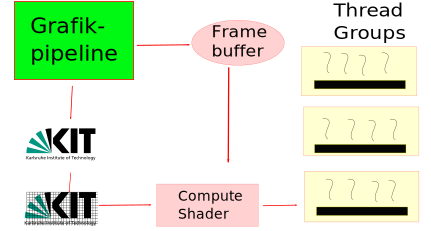
\includegraphics[width=\linewidth]{Bilder/ComputeShader.pdf}
            \label{Compute Shader}
            \caption{Funktionsweise Compute Shader}
        \end{minipage}
        \hfill
        \begin{minipage}[t]{0.45\linewidth}
            \centering
            \includegraphics[width=\linewidth]{Bilder/GeometryBlur.png}
            \caption{Postprocessing Blur mit Compute Shader~\cite{computeBlur}}
        \end{minipage}
    \end{figure}

    Die erste Abbildung zeigt nochmal deutlich, dass der Compute Shader für jedwedige Art der Berechnung eingesetzt werden kann, bei dem \textit{stream processors} 
    zu tragen kommen. Eine Beobachtung war die effiziente Verlegung der Mesh Verarbeitung auf den Compute Shader. Dies führte zu der Einführung von 
    Mesh Shadern~\ref{sec:Meshshader}, die stark an dem Aufbau von Compute Shadern orientiert sind.

\chapter{Unterschied moderne und klassische Rendering-Pipeline}

    Über die vielen Jahre, in denen sich die Grafikpipeline entwickelt hat, kann man eine lange Entwicklungsphase von einer konfigurierbaren
    zu einer immer mehr und mehr freiprogrammierbaren Pipeline ausmachen.
    Hardwareunterschiede früher bei Shadern <--> gleiche bauart, flexible aufteilung je nach anwendungsgebiet(unified shaders);
    früher keine geometry shader; diese wurden eingeführt um Last von der CPU auf die GPU auszulagern; FPC wachsen viel schneller mit GPU
    als bei CPU; haben sich sogar weiterhin als zu unflexibel erwiesen; sehr aktuelle Entwicklungen zeigen weiterentwicklung~\ref{sec:Meshshader};
    weil lacken bei einem Thread abarbeitung!!! geometry shader konzept!!!

    \section{Freie Programmierung oder reines Konfigurieren}
        
        \begin{figure}[H]
            \centering
            \begin{minipage}[t]{0.45\linewidth}
                \centering
                \def\svgwidth{\columnwidth}
                \import{Bilder/}{AltesOpenGL.pdf_tex}
                \label{Altes OpenGL}
                \caption{OpneGL $\leq$ 2.0}
            \end{minipage}
            \hfill
            \begin{minipage}[t]{0.45\linewidth}
                \centering
                \def\svgwidth{\columnwidth}
                \import{Bilder/}{ModernesOpenGL.pdf_tex}
                \label{Modernes OpenGL}
                \caption{Modernes OpenGL}
            \end{minipage}
        \end{figure}

    \section{Vertex Arrays, Index Buffers, ..}

%% ===============================================================================================================================
\chapter{Ausblick}

\section{Raytracing Unterstützung}
\label{sec:Real-Time Raytracing}
In heutigen modernen Grafikprogrammierschnittstellen(Vulkan, DirectX) befindet sich Raytracing-Funktionalität.
Raytracing Ansätze gehen von der objektbasierten (siehe Rasterisierung) zu der Image-ordered Bilderstellung über.
Hiermit werden nicht nur Primär- sondern auch Sekundärstrahlen(etc.) betrachtet und somit unter Anderem Schatten und Spiegelungen.
Wir können diese neuen Shader wie Compute Shader~\ref{sec:Compute Shader} programmieren.

\begin{center}
    \begin{table}[H]
        \begin{tabular}{ | l | p{10cm} |}
        \hline
        Shader        &  Beschreibung \\ \hline
        Any Hit       &  Kann ausgeführt werden wenn wir einen Schnitt mit unserem Strahl gefunden haben. Soll bei transparenten Objekten dazu führen,
                        früher abbrechen zu können.\\ \hline
        Callable      &  Kann von einem anderen Shader aufgerufen werden.\\ \hline
        Closest Hit   &   Wird ausgeführt wenn ein Standardstrahl von einem Ray Generation Shader verschossen wurde, und ein "nähster Schnittpunkt"
                        gefunden wurde. Hier kann der Programmierer die Methode \textit{shade()} implementieren. Dabei sollte auf Schatten getestet, 
                        weitere Reflektions- und Transmission miteinberechnet werden\\ \hline
        Intersection  &   Wird aufgerufen, falls wir eine Bounding Box unser Beschleunigungsstruktur treffen.\\ \hline
        Miss          &   Wird aufgerufen, falls keine Szenengeometrie getroffen wurde.\\ \hline
        Ray Generation&   Mit \textit{TraceRay()} können wir Strahlen verschießen. Normalerweiße versendet man einen Strahl pro Pixel.
                        Wir können jedwedigen Typ von Strahl damit verschießen(Schatten, Primär, Transmit)\\ \hline
        \hline
        \end{tabular}
        \caption{Shadereinheiten nach DirectX12.}
    \end{table}
\end{center}

Hierbei führt ein verschossener Strahl eine Datenstruktur("\textit{payload}") mit sich, die eine variable Menge an Informationen
speichern kann. Als wichtigste zu nennen ist die Distanz bei einem Hit.\par
Aktuelle Bemühungen gehen nun daran Raytracing und Rasterisierung zu kombinieren. Barr$\acute{e}$-Brisebois \cite{Barré-Brisebois2019} stellte
mit dem Spiel \textit{PICA PICA} eine solche Rendering-Pipeline vor, welche mithilfe von Path Tracing arbeitet. Dabei wird der G-Buffer
(Texturen die Position, Normalen, Belichtung eines Frames speichern) noch über Rasterisierung berechnet. Direkten Schatten kann man 
rastern oder raytracen. Diese Option verspricht eine Anpassungsfähigkeit der Pipeline nach Leistungsfähigkeit. Ähnlich können nun
Reflektionen, Global Illumination, Ambient Occlusion und Transmission geraytraced oder auf Compute Shader ausgeführt werden.(Wieder je nach 
Hardwareleistung). Einzig direkte Beleuchtung sowie Post-Processing Effekte laufen nur über Compute-Shader.

\section{Task-/Mesh Shaders}
\label{sec:Meshshader}
Der aktuelle Trend bei der Modellerstellung geht über zu immer komplexeren Modellen. Dabei stößt die traditionelle Pipeline mit der 
enormen Anzahl von Dreiecken an ihre Grenzen. Die damalige Einführung des Tessellation~\ref{subsec:Tessellation}- und des Geometryshaders~\ref{subsec:Geometry Shader}
(vorallen aber Tessellation!) war aus selbigen Grund und brachte eine erwünschte Weitung des Flaschenhalses und bessere Arbeitsaufteilung
innerhalb der Pipeline. Das obige besprochene Primitive Assembly~\ref{subsec:Primitive Assembly} erweist sich als \textit{Fixed Function} innerhalb
der Pipeline als zu star und unflexibel. Für starre Szenen wird hohe Bandbreite veranschlagt, da wir unseren Index Buffer jedesmal berechnen müssen.
Anstatt wie beim Primitive Assembly~\ref{subsec:Primitive Assembly} von der Hardware das Vertex Array Objekt aufs neue Berechnen zu lassen, teilt 
man nun die Geometrie selbst in \textit{Meshlets} auf und speichert diese in einen Buffer(\textit{Meshlet Desc Buffer}), wobei jedes \textit{Meshlet} 
für sich auf einen VBO zeigt (Man hält den Buffer \textit{On-Chip}; ähnlich Compute Shader Model~\ref{sec:Compute Shader}). 
Diese Aufteilung gibt uns ein besseres Wiederverwenden der Eckpunkte und daher wird Bandbreite gespart!
Die Mesh Shader kommen nach dem Compute Shader Model~\ref{sec:Compute Shader} und lassen eindeutig den Trend von fixen Vorgängen innerhalb der Pipeline 
zu mehr Flexibleren wiedererkennen. Durch diese freie Programmiermöglichkeit ergeben sich vielfältige Möglichkeiten, so z.B. für \textit{Mesh compression} 
da sich die Buffer selber beschreiben lassen. 

\begin{figure}[H]
    \centering
    \includegraphics[width=1.\textwidth]{Bilder/meshlets_pipeline.png}
    \caption{Vergleich bisherige Vertex,Tessellation,Geometry Pipeline <--> \textit{stream procesor artig} Mesh Shader Pipeline}
\end{figure}

Dabei arbeitet der Task Shader ähnlich der Tessellation Control Einheit~\ref{subsec:Tessellation} und verteilt zunächst das Mesh in \textit{workgroups}.
Jedoch ist anzumerken, dass der Task Shader mit einem kooperativen Threadmodell arbeitet und dessen In-/Output komplett frei programmierbar ist.
Man ist nicht mehr auf ein ankommendes Primitiv und eine ausgehende Tessellation Entscheidung beschränkt. Damit lassen sich Level of Detail Entscheidungen
treffen, also wie fein unterteile ich mein einkommendes Primitiv. Oder man entscheidet sogar eine Gruppe gar nicht zu zeichnen (Culling) und schickt 
keine weitere Arbeit weiter.
Der Mesh Shader nimmt lediglich die \textit{workgroup id} entgegen und arbeitet ähnlich dem Compute Shader~\ref{sec:Compute Shader} auf einer Threadgruppe
(hier langt jedoch ein eindimensionales Array). Es gibt hier jedoch nicht nur einen gemeinsamen Speicher, sondern auch einen Output, welcher frei-programmierbar ist. 
Zum Geometry Shader, der keine Threadgruppe besitzt, ist dies ein großer Schritt.

%% ========================================================================================================================================

%% content.tex
%%
